% Source: graduate-coursework/Prior_Semesters/Fa25/EMCH501/HW2/HW2.tex

\documentclass[border=4pt]{standalone}
\usepackage{amsmath}
\usepackage{amssymb}
\usepackage{graphicx}
\usepackage{tikz}
\usepackage{xcolor}
\usetikzlibrary{shapes.geometric, arrows.meta, positioning, decorations.pathmorphing, patterns}

\begin{document}
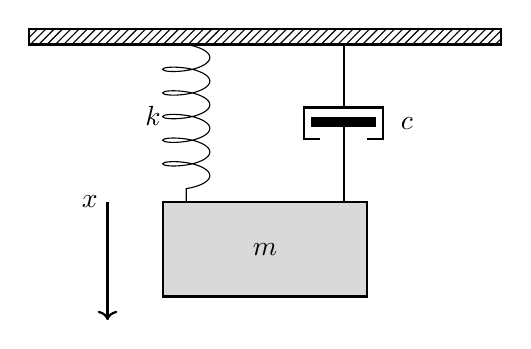
\begin{tikzpicture}[scale=1.0]
  % ceiling
  \draw[thick,pattern=north east lines] (-3,2) rectangle (3,2.2);
  \draw[thick] (-3,2) -- (3,2);
  % spring (left side)
  \draw[decoration={coil,aspect=0.3,segment length=3mm,amplitude=3mm},decorate] (-1,2) -- (-1,0.0);
  \node[left] at (-1.2,1.1) {$k$};
  % damper (right side)
  \draw[thick] (1,2) -- (1,1.2); % top rod
  \draw[thick] (1.3,0.8) -- (1.5,0.8) -- (1.5,1.2) -- (0.5,1.2) -- (0.5,0.8) -- (0.7,0.8); % housing
  \draw[thick,fill=black] (0.6,1.07) rectangle (1.4,0.97); % piston
  \draw[thick] (1,1.0) -- (1,0); % bottom rod
  \node[right] at (1.6,1.0) {$c$};
  % connecting bar at top of mass
  \draw[thick] (-1.3,0) -- (1.3,0);
  % mass
  \draw[fill=gray!30,thick] (-1.3,0) rectangle (1.3,-1.2);
  \node at (0,-0.6) {$m$};
  % coordinate system
  \draw[->,thick] (-2,0) -- (-2,-1.5);
  \node[left] at (-2,0) {$x$};
\end{tikzpicture}
\end{document}
